\section{Implementácia}
\label{sec:impl}

% ----- Použité technológie -----
\subsection{Použité technológie}

Použité technológie sú zhrnuté v Tab.~\ref{tab:tech}.

% Tabuľka: Použité technológie.
\begin{table}[ht]
  \centering
  \small
  \caption{Použité technológie.}
  \label{tab:tech}
  \begin{tabularx}{\textwidth}{|l|Y|}
    \hline
    \rowcolor[gray]{0.9} \textbf{Časť} & \textbf{Technológia} \\
    \hline
    Klient & React, Vite, čisté CSS (bez knižnice komponentov) \\
    \hline
    Server & Python, FastAPI, Uvicorn \\
    \hline
    Spracovanie dát & pandas \\
    \hline
    Úložisko & SQLite (súbor \code{backend/sessions.sqlite3}) \\
    \hline
  \end{tabularx}
\end{table}

% ----- Klientska aplikácia -----
\subsection{Klientska aplikácia}

Zdrojový kód klienta je v priečinku \code{src/}. Aplikácia je rozdelená na
obrazovky, opakovane použiteľné komponenty, hooky a pomocné funkcie:

\begin{itemize}
  \item \code{App.jsx} riadi prechody medzi stavmi (\code{setup},
        \code{run}, \code{identify}, \code{done}) a drží
        údaje relácie vrátane zvoleného režimu,
  \item \code{constants.js} definuje režimy písania (\code{MODES}: veta
        a slovo s textom a popiskami), počet opakovaní a ignorované
        a opravné klávesy,
  \item \code{components/} obsahuje obrazovky (\code{setup}, \code{run},
        \code{identify}, \code{done}) a spoločné časti karty
        s písaním (\code{typing}): zobrazenie textu s kurzorom, skryté vstupné pole, hlavičku
        a graf rytmu,
  \item \code{hooks/useTypingAttempt.js} zaznamenáva udalosti jedného
        pokusu a používajú ho obrazovky merania aj identifikácie,
  \item \code{hooks/usePressedKeys.js} sleduje stlačené klávesy na
        zvýraznenie klávesnice v pozadí,
  \item \code{hooks/useRandomKeys.js} na úvodnej obrazovke náhodne
        „stláča“ klávesy pozadia ako ukážkovú animáciu (vypína sa pri
        nastavení systému \emph{znížený pohyb}),
  \item \code{utils/} obsahuje volania API, export do CSV, výpočet súhrnu,
        text hlásení o chybe (\code{mistake.js}) a zisťovanie dotykového
        zariadenia (\code{device.js}),
  \item \code{styles/} obsahuje štýly rozdelené podľa obrazovky.
\end{itemize}

Hook \code{useTypingAttempt} registruje poslucháčov \code{keydown} a
\code{keyup} priamo na (skrytom) vstupnom poli. Pri stlačení uloží udalosť
a vytvorí úsečku grafu rytmu, pri uvoľnení doplní jej koniec. Po stlačení
klávesu Enter zavolá funkciu, ktorú mu odovzdala obrazovka (pokus
sa overí a buď zapíše, alebo zamietne). Hook dostane aj cieľový text
(\code{target}). Pri stlačení Backspace alebo Delete (kláves sa vtedy
nevykoná) a pri znaku, po ktorom napísaný text už nie je začiatkom cieľového
textu, hook pokus nezruší hneď: na 1,6~s zamkne vstup a vráti objekt
\code{mistake} (druh chyby, napísaný a očakávaný znak). Obrazovka z neho
zloží hlásenie (\code{utils/mistake.js}), trasie zobrazeným textom a po
uplynutí času sa pokus vynuluje. Údaje o pokusoch sa
držia v referenciách, aby zápis udalostí nespôsoboval zbytočné
prekresľovanie; stav (\code{useState}) sa mení len pre text a úsečky grafu.

Počas merania sa v reálnom čase kreslí graf rytmu na plátno
\code{canvas} (Obr.~\ref{fig:run}): oranžové úsečky patria aktuálnemu
pokusu a zlaté predchádzajúcemu. Pozadie tvorí stylizovaná klávesnica, ktorá
zvýrazňuje práve stlačené klávesy a nemá vplyv na meranie.
Obrazovka prípravy relácie je na Obr.~\ref{fig:setup}.

Dynamika písania sa meria len na fyzickej klávesnici. Dotykové klávesnice
telefónov často posielajú udalosti s \code{key = "Unidentified"} a ich časy
sú nepresné, preto \code{utils/device.js} pri štarte zistí dotykové zariadenie
a \code{App.jsx} namiesto aplikácie zobrazí hlásenie „Nie je podporované“.
Zariadenie sa rozpozná podľa \code{userAgentData.mobile}, reťazca
\emph{User-Agent} a podľa vlastností obrazovky (\code{pointer: coarse},
\code{hover: none} a viac dotykových bodov), takže ho nezmení ani voľba
„zobrazenie pre PC“ v prehliadači. Ide len o upozornenie, nie o bezpečnostnú
ochranu. Úvodná obrazovka je na počítačoch pevná (bez posúvania stránky).

% Obrázok (obrázok zo súboru figures/ui-setup.png): Obrazovka prípravy relácie.
\begin{figure}[ht]
  \centering
  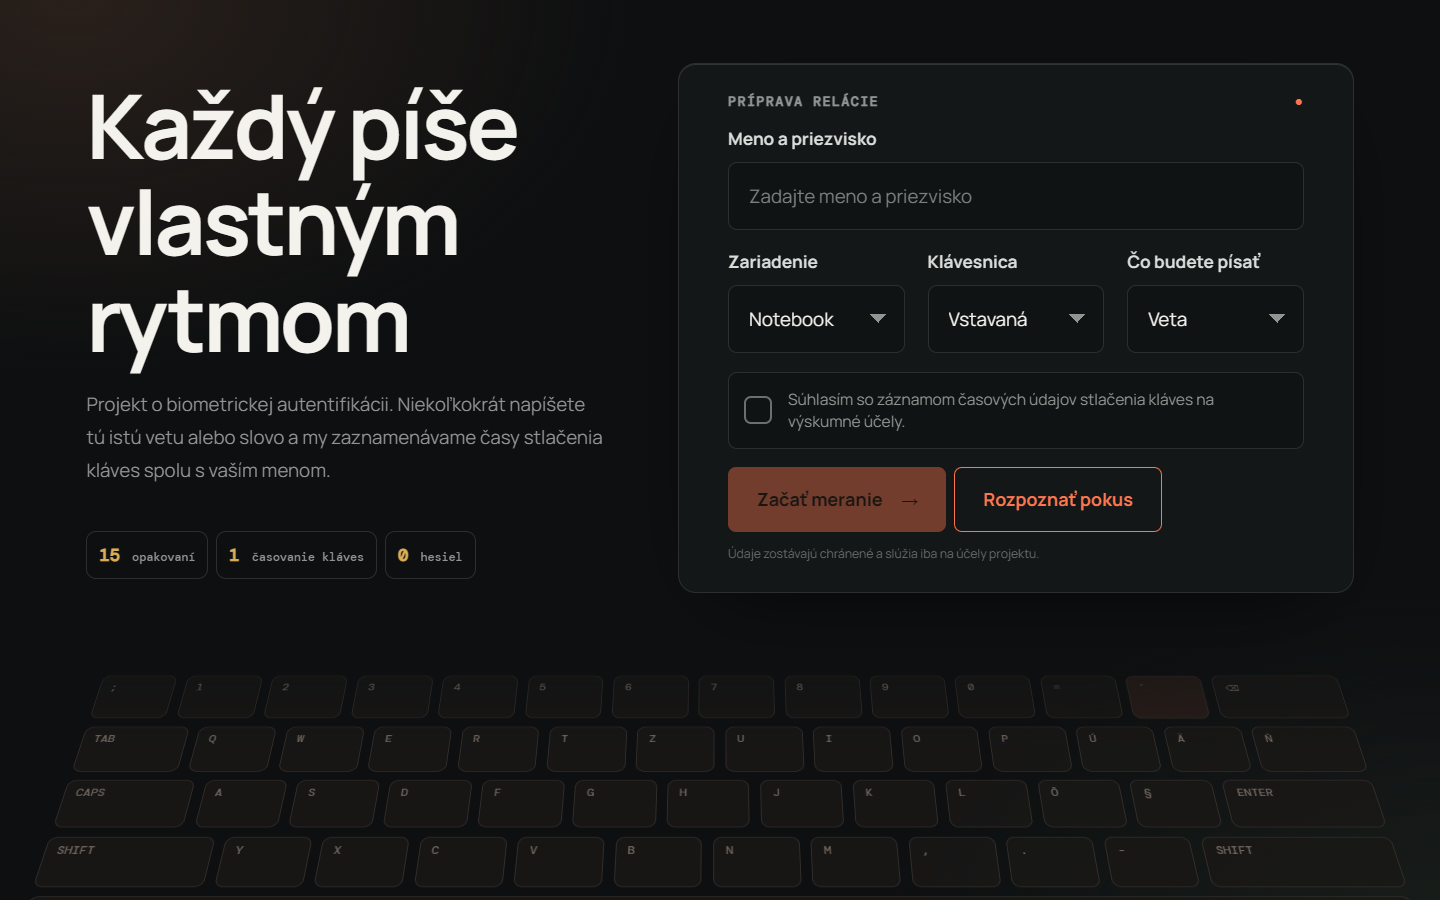
\includegraphics[width=\textwidth]{ui-setup.png}
  \caption{Obrazovka prípravy relácie.}
  \label{fig:setup}
\end{figure}

% Obrázok (obrázok zo súboru figures/ui-run.png): Obrazovka merania: veta, vstupné pole a graf rytmu.
\begin{figure}[ht]
  \centering
  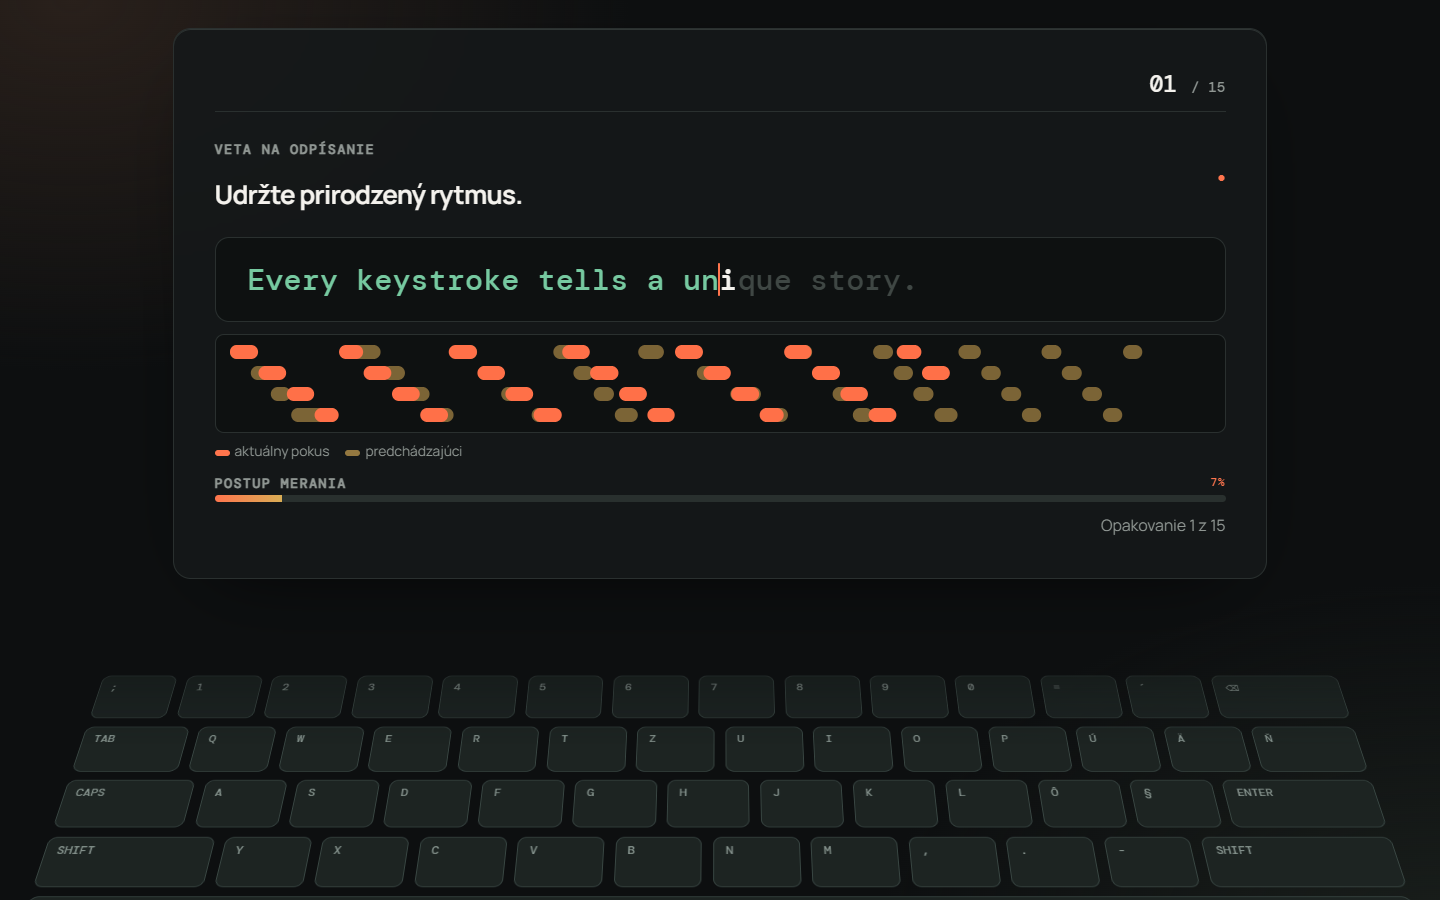
\includegraphics[width=\textwidth]{ui-run.png}
  \caption{Obrazovka merania: veta, vstupné pole a graf rytmu.}
  \label{fig:run}
\end{figure}

% ----- Serverová časť -----
\subsection{Serverová časť}

Server (\code{backend/main.py}) poskytuje rozhranie REST uvedené v
Tab.~\ref{tab:api}. Dokumentácia vo formáte OpenAPI je dostupná na
adrese \code{/docs}.

% Tabuľka: Koncové body API.
\begin{table}[ht]
  \centering
  \small
  \caption{Koncové body API.}
  \label{tab:api}
  \begin{tabularx}{\textwidth}{|l|l|Y|}
    \hline
    \rowcolor[gray]{0.9} \textbf{Metóda} & \textbf{Cesta} & \textbf{Popis} \\
    \hline
    GET  & \code{/api/health} & kontrola dostupnosti \\
    \hline
    POST & \code{/api/sessions} & uloženie dokončenej relácie \\
    \hline
    GET  & \code{/api/sessions} & zoznam relácií bez udalostí (\code{limit}, \code{offset}) \\
    \hline
    GET  & \code{/api/sessions/\{id\}} & metadáta a všetky udalosti jednej relácie \\
    \hline
    GET  & \code{/api/stats} & počet relácií a udalostí \\
    \hline
    POST & \code{/api/identify} & identifikácia jedného pokusu (\code{rows}, \code{mode}) \\
    \hline
    GET  & \code{/api/evaluation} & vyhodnotenie na pokusoch 11--15 (voliteľný parameter \code{mode}) \\
    \hline
    GET  & \code{/api/compare} & porovnanie režimov veta a slovo \\
    \hline
  \end{tabularx}
\end{table}

Relácie sa ukladajú do tabuľky \code{sessions} so stĺpcami \code{id},
\code{participant\_id}, \code{session\_id}, \code{meta\_json},
\code{rows\_json} a \code{created\_at}. Udalosti celej relácie sú uložené
ako jeden JSON dokument. Uloženie je idempotentné: ak už existuje relácia
s rovnakým \code{session\_id}, server nič nezapíše a vráti stav
\code{already\_saved}. Pri chýbajúcom \code{participant\_id},
\code{session\_id}, prázdnom zozname udalostí alebo neznámom režime vráti
chybu 422. Počet kláves v pokuse určuje slovník \code{MODE\_KEYS}
(\code{phrase}: 37, \code{word}: 10), takže validácia a príznaky sa riadia
režimom; relácie bez poľa \code{mode} sa čítajú ako \code{phrase}.

Po každom novo uloženom zázname server na pozadí (\code{BackgroundTasks})
prekreslí súbor \code{accuracy\_chart.png} knižnicou matplotlib: stĺpcový graf
top-1 a top-3 pre vetu a slovo, vypočítaný rovnako ako \code{/api/compare}.
Odpoveď na uloženie sa tým nespomalí a zlyhanie kreslenia uloženie neovplyvní.

% ----- Známe obmedzenia implementácie -----
\subsection{Známe obmedzenia implementácie}
\label{sec:obmedzenia}

Pri interpretácii výsledkov treba zohľadniť tieto obmedzenia:
\begin{itemize}
  \item Pokusy s opravou klávesom Backspace alebo Delete server pri tvorbe
        šablón ignoruje (majú viac ako $n$ stlačení). Klient takéto pokusy
        už nepripustí, no v skorších reláciách sa ešte nachádzajú.
  \item Zariadenie a typ klávesnice sa ukladajú len ako metaúdaje a do
        výpočtov nevstupujú.
  \item Šablóny sa pri každej požiadavke na identifikáciu alebo vyhodnotenie
        počítajú nanovo zo všetkých relácií daného režimu. Pre malý počet
        účastníkov to stačí, pri väčšom objeme dát by bolo vhodné šablóny
        ukladať.
  \item Pri troch a menej účastníkoch je metrika top-3 triviálne rovná
        100\,\%, keďže zoznam obsahuje všetkých účastníkov.
  \item Identifikátorom účastníka je zadané meno, takže databáza obsahuje
        osobné údaje a nemá sa verzionovať ani zverejňovať.
  \item Závislosti klienta sú v \code{package.json} uvedené ako
        \code{latest}; reprodukovateľnosť zaisťuje súbor
        \code{package-lock.json}, v \code{requirements.txt} sú uvedené
        len dolné hranice verzií.
\end{itemize}

% ----- Ukážky kľúčového kódu -----
\subsection{Ukážky kľúčového kódu}

Výpočet vektora príznakov z jedného pokusu (\code{backend/main.py}, skrátené):

\begin{lstlisting}[language=Python]
# 1. Udalosti pokusu zoradíme a rozdelíme na stlačenia a uvoľnenia
frame = pd.DataFrame(rows).sort_values("seq")
downs = frame[frame["event"] == "down"]
ups = frame[frame["event"] == "up"]

# 2. Platný pokus má presne key_count stlačení a uvoľnení
#    (key_count = MODE_KEYS[mode]: 37 pre vetu, 10 pre slovo)
if len(downs) != key_count or len(ups) != key_count:
    raise ValueError(f"an attempt must contain exactly {key_count} key presses and releases")
...

# 3. Doba držania = čas uvoľnenia mínus čas stlačenia tej istej klávesy
holds = []
for _, down in downs.iterrows():
    matching = ups[(ups["code"] == down["code"]) & (ups["seq"] > down["seq"])]
    holds.append(float(matching.iloc[0]["t_ms"]) - float(down["t_ms"]))

# 4. Interval = rozdiel časov dvoch po sebe idúcich stlačení
intervals = [down_times[i] - down_times[i - 1] for i in range(1, len(down_times))]

# 5. Vektor príznakov: n dôb držania + (n-1) intervalov (veta: 73, slovo: 19)
return holds + intervals
\end{lstlisting}

Šablóna účastníka a vzdialenosť nového pokusu od nej:

\begin{lstlisting}[language=Python]
# Každý riadok matice je jeden platný pokus (2n-1 príznakov), pokusy 1-10 jedného režimu
matrix = pd.DataFrame(vectors)

# Šablóna účastníka: priemer a smerodajná odchýlka každého príznaku
mean = matrix.mean().tolist()
std = matrix.std(ddof=0).replace(0, 1).tolist()   # nulová odchýlka -> 1
...

# Vzdialenosť nového pokusu od šablóny (štandardizovaná euklidovská)
distance = sqrt(sum(((v - c) / s) ** 2 for v, c, s in zip(vector, mean, std)))
...

# Neznámy pokus: priemerná odchýlka na jeden príznak je väčšia ako 3
unknown = best_distance / sqrt(len(vector)) > 3
\end{lstlisting}
